
\section{AXOL1TL and TOPO model names}

This document is a description for the naming convention of AXOL1TL and TOPO model names.

With the release of utm version 0.12, the possibility of setting cuts for different models of AXOL1TL and Topological triggers is available.
To prevent changes in utm and TME, we created a structure which is open for upcoming new models without changes in utm and/or TME!\\
The uGT tool "VHDL Producer" and the uGT firmware (VHDL) code depend on the AXOL1TL and TOPO model names. Therefore a convention is necessary.\\
A list of valid AXOL1TL and TOPO model names will be provided on a web page (an example is available \url{https://globaltrigger.web.cern.ch/upgrade/tme/models}).

\subsection{Implementation in Trigger Menu Editor (TME)}

In TME "cut editor" a link to valid model names is available for L1Menu developers to set model names according to this convention, see Figure \ref{fig:tme_model_cut} for an example of Topological trigger (similar for AXOL1TL trigger).

\begin{figure}[htb]
\centering
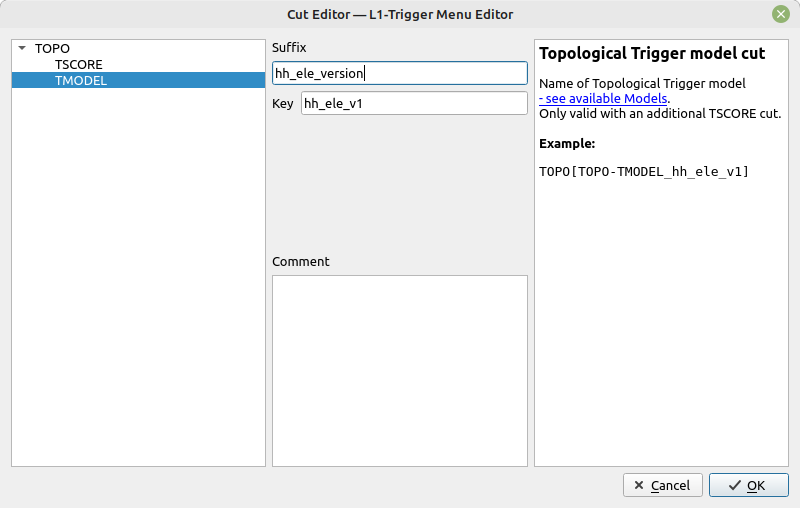
\includegraphics[width=15cm]{figures/tme_model_cut}
\caption{TME cut editor - MODEL for Topological trigger}
\label{fig:tme_model_cut}
\end{figure}

\subsection{Implementation in uGT firmware}

The uGT firmware (\url{https://github.com/cms-l1-globaltrigger/mp7_ugt_legacy}) will provide subdirectories for HLS generated VHDL files of every available model.\\
According to the model names listed in \url{https://globaltrigger.web.cern.ch/upgrade/tme/models}, we created a subdirectory structure as follows (an example of the structure is currently in branch "dev\_v1.26.x\_nn\_models" - \url{https://github.com/cms-l1-globaltrigger/mp7_ugt_legacy/tree/dev_v1.26.x_nn_models/firmware/hdl/payload/gtl}):

\texttt{../axol1tl\_trigger/model\_v1}\\
containing VHDL files named "axol1tl\_v1\_<hls file name>.vhd" and "axol1tl\_v1.vhd".\\\\
\texttt{../axol1tl\_trigger/model\_v3}\\
containing VHDL files named "axol1tl\_v3\_<hls file name>.vhd" and "axol1tl\_v3.vhd".\\\\
\texttt{../topo\_trigger/model\_hh\_ele\_v1}\\
containing VHDL files named "topo\_hh\_ele\_v1\_<hls file name>.vhd" and "topo\_hh\_ele\_v1.vhd". (See example Figure \ref{fig:hh_ele_v1_files}).\\\\
\texttt{../topo\_trigger/model\_hh\_had\_v1}\\
containing VHDL files named "topo\_hh\_had\_v1\_<hls file name>.vhd" and "topo\_hh\_had\_v1.vhd".\\\\
\texttt{../topo\_trigger/model\_hh\_mu\_v1}\\
containing VHDL files named "topo\_hh\_mu\_v1\_<hls file name>.vhd" and "topo\_hh\_mu\_v1.vhd".\\

VHDL file names and VHDL entity names of HLS generated files have to comply with this naming convention.\\
An example of HLS generated files is shown in Figure \ref{fig:hh_ele_v1_files} (for Topological trigger model "hh\_ele\_v1").

\begin{figure}[htb]
\centering
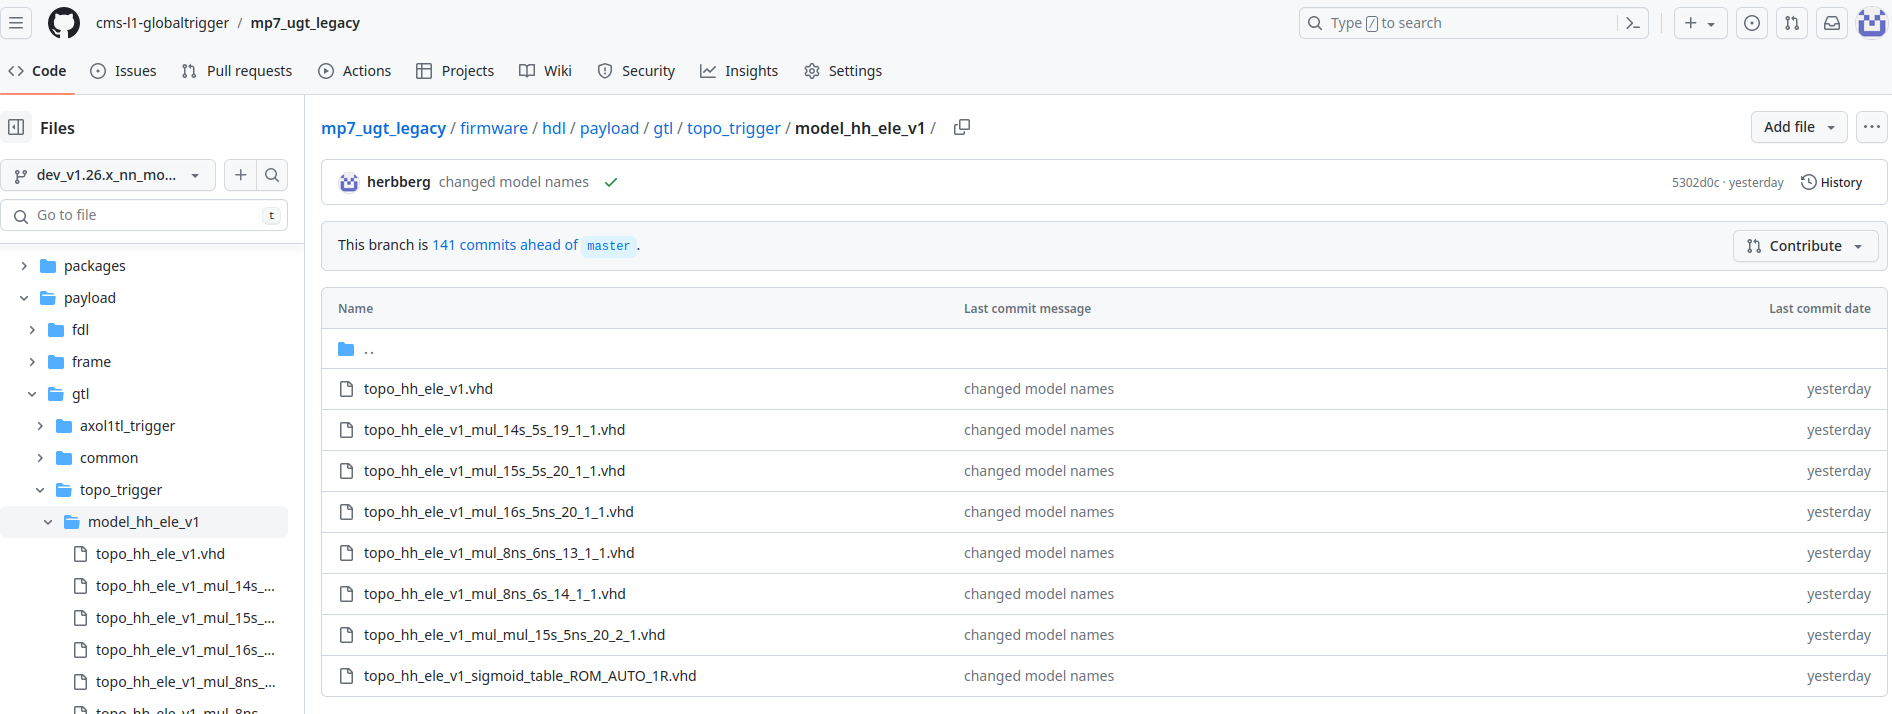
\includegraphics[width=15cm]{figures/hh_ele_v1_files}
\caption{TOPO model "hh\_ele\_v1" files}
\label{fig:hh_ele_v1_files}
\end{figure}

The dependency files \texttt{axol1tl\_trigger.dep} and \texttt{topo\_trigger.dep} should contain all HLS generated filenames (with path) for all models.\\
In Figure \ref{fig:topo_dep} an example for \texttt{topo\_trigger.dep} is shown.\\

The current implementation for "Anomaly Detection Trigger" (ADT) will be available, too (it contains the logic of model "v3").\\

Developers of AXOL1TL and Topological trigger firmware should make PR for their HLS generated VHDL files in the model directories at \url{https://github.com/cms-l1-globaltrigger/mp7_ugt_legacy/tree/dev_v1.26.0/firmware/hdl/payload/gtl} for first tests. In the case of new model please create a new subdirectory named \texttt{model\_<new model name>} with the new VHDL files and create a PR for it. All the new VHDL files (path) of the new model must be appended to \texttt{axol1tl\_trigger.dep} or \texttt{topo\_trigger.dep}. The "wrapper" file (similar to e.g. \texttt{axol1tl\_v3\_wrapper.vhd}) will be created by uGT.\\

\begin{figure}[htb]
\centering
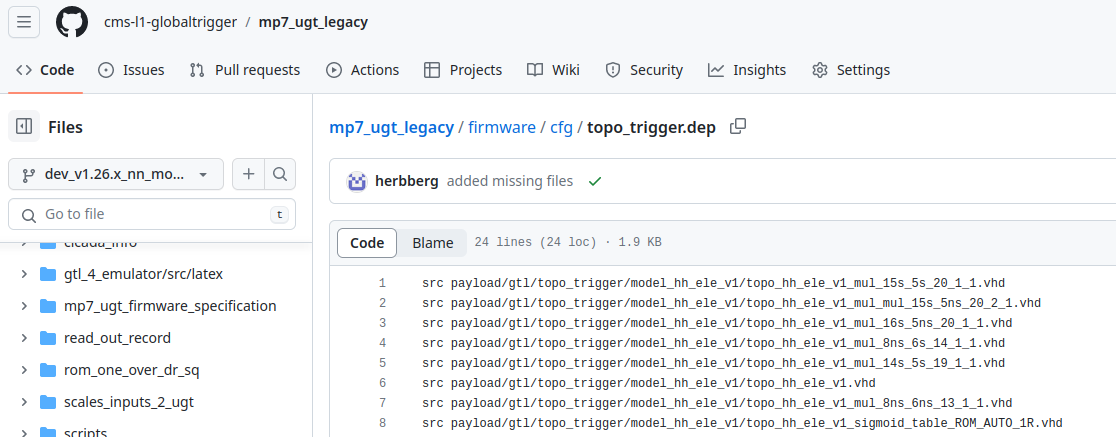
\includegraphics[width=15cm]{figures/topo_dep}
\caption{Example of \texttt{topo\_trigger.dep} (for model "hh\_ele\_v1" files)}
\label{fig:topo_dep}
\end{figure}
